\subsection{What does the agent learn?}\label{sec:behaviour}
Figure~\ref{fig:behaviour} shows how actions and latent states evolve through the day, aggregated over the 500 test days (and over the ten seeds for AA-DQN). Three behavioural regularities distinguish the learned policy from the heuristics.

\emph{Work while fresh.} AA-DQN almost never rests in the first hour (0.5\% of slots, versus 3.6\% for SPT-Threshold, 4.6\% for EDF-Threshold and a fixed 16.7\% for EDF-Periodic). It exploits the high morning attention and lets fatigue rise to $\approx\!0.38$ before it starts to insert breaks. A fixed cycle cannot distinguish a fresh worker at 09:30 from a recovered one at 15:00, and a threshold rule reacts only once a threshold has been crossed.

\emph{Rest when work is least productive.} The break share of AA-DQN rises to a peak of 24.6\% between 13:00 and 14:00, which coincides with the modelled post-lunch dip, and declines afterwards. In the 13:00--15:00 window it rests in 22.4\% of slots, versus 12.5\% at other times. Resting is cheapest when the productivity it forgoes is lowest (Eq.~\eqref{eq:rho}). The threshold rules show a similar but sharper peak (35--36\% between 13:00 and 14:00) only because the dip pushes observed attention below their fixed threshold.

\emph{Match difficulty to capacity without starving hard tasks.} AA-DQN devotes about half of the morning slots to hard tasks (50\% at 09:00--11:00), reduces this to one third around the afternoon trough (33\% at 13:00--15:00), and returns to hard work in the last hour (48\%) as their deadlines approach. SPT-Threshold behaves very differently. It does almost no hard work in the first hour (8\%) because hard tasks are long, postpones them until they become urgent, and then spends 82\% of the last hour on hard work, when attention is lowest and hard tasks are slowest (Eq.~\eqref{eq:rho}). This back-loading explains its low difficulty-weighted on-time rate (Section~\ref{sec:main}). EDF, in contrast, does more hard work in the afternoon (71\%) than in the morning (60\%) and never rests. The hand-crafted Cog-Heuristic was designed to capture the difficulty--attention intuition but, with a single attention threshold, also pushes hard tasks into the late afternoon (67\% after 16:00). The learned policy is the only one that front-loads demanding work while still finishing short tasks, which illustrates how hard it is to encode such time-, state- and deadline-dependent trade-offs in rules.

Compared with the memoryless DQN, AA-DQN rests more (\AADQNBreakPct\% versus \DQNBreakPct\% of slots) and takes breaks at a lower true fatigue level (0.36 versus 0.44). The DQN concentrates its rest in the last hour (29\% of slots after 16:00), consistent with late, reactive breaks triggered by single noisy readings.

\begin{figure}[!htbp]
\centering
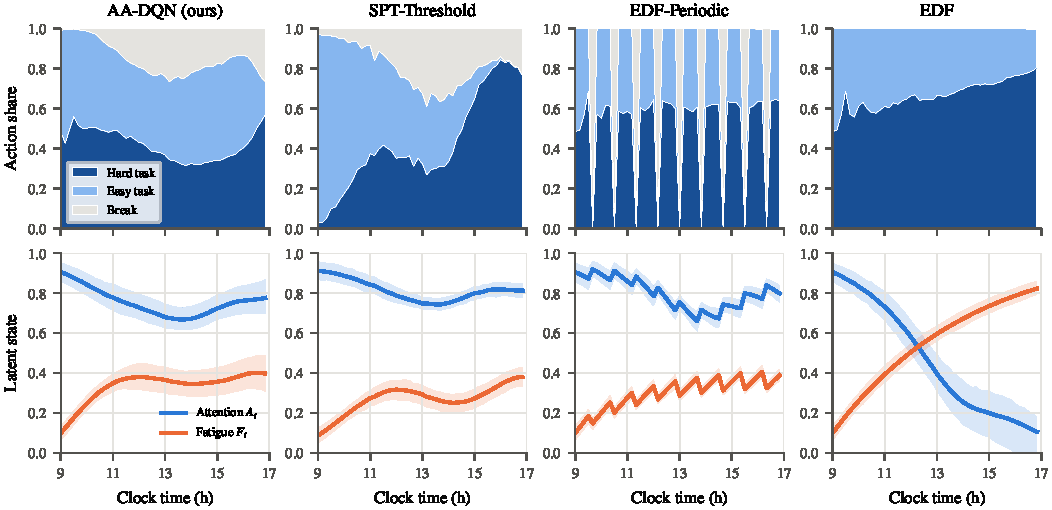
\includegraphics[width=\textwidth]{figures/fig_behaviour.pdf}
\caption{Learned and heuristic behaviour across the workday on 500 test days. Top: share of slots spent on hard tasks, easy tasks and breaks. Bottom: mean true attention and fatigue (bands: interquartile range). The saw-tooth pattern of EDF-Periodic reflects its fixed work--rest cycle.}
\label{fig:behaviour}
\end{figure}
